\documentclass[a4paper, 14pt]{extarticle}

% Поля
%--------------------------------------
\usepackage{geometry}
\usepackage{float}
\geometry{a4paper,tmargin=2cm,bmargin=2cm,lmargin=3cm,rmargin=1cm}
%--------------------------------------


%Russian-specific packages
%--------------------------------------
\usepackage[T2A]{fontenc}
\usepackage[utf8]{inputenc} 
\usepackage[english, main=russian]{babel}
%--------------------------------------
\usepackage{textcomp}

% Красная строка
%--------------------------------------
\usepackage{indentfirst}               
%--------------------------------------             


%Graphics
%--------------------------------------
\usepackage{graphicx}
\graphicspath{{./images/}{./}}
\usepackage{wrapfig}
%--------------------------------------

% Полуторный интервал
%--------------------------------------
\linespread{1.3}                    
%--------------------------------------

%Выравнивание и переносы
%--------------------------------------
\sloppy
\clubpenalty=10000
\widowpenalty=10000
%--------------------------------------

%Списки
\usepackage{enumitem}

%Подписи
\usepackage{caption} 

%Гиперссылки
\usepackage{hyperref}
\hypersetup { unicode=true }
\usepackage{tikz}
\usetikzlibrary{arrows.meta, positioning, shapes.geometric}

%Рисунки
%--------------------------------------
\DeclareCaptionLabelSeparator*{emdash}{~--- }
\captionsetup[figure]{labelsep=emdash,font=onehalfspacing,position=bottom}
%--------------------------------------

% НАСТРОЙКИ ДЛЯ РУССКОГО ЯЗЫКА В LISTINGS
%--------------------------------------
\usepackage{listings}
\usepackage{xcolor}

\lstset{
  belowcaptionskip=1\baselineskip,
  breaklines=true,
  frame=L,
  xleftmargin=\parindent,
  language=Python,
  showstringspaces=false,
  basicstyle=\footnotesize\ttfamily,
  keywordstyle=\bfseries\color{blue},
  commentstyle=\itshape\color{purple},
  identifierstyle=\color{black},
  stringstyle=\color{red},
  inputencoding=utf8,
  extendedchars=true,
  literate=
    {а}{{\selectfont\char224}}1 {б}{{\selectfont\char225}}1 {в}{{\selectfont\char226}}1
    {г}{{\selectfont\char227}}1 {д}{{\selectfont\char228}}1 {е}{{\selectfont\char229}}1
    {ё}{{\"e}}1 {ж}{{\selectfont\char230}}1 {з}{{\selectfont\char231}}1
    {и}{{\selectfont\char232}}1 {й}{{\selectfont\char233}}1 {к}{{\selectfont\char234}}1
    {л}{{\selectfont\char235}}1 {м}{{\selectfont\char236}}1 {н}{{\selectfont\char237}}1
    {о}{{\selectfont\char238}}1 {п}{{\selectfont\char239}}1 {р}{{\selectfont\char240}}1
    {с}{{\selectfont\char241}}1 {т}{{\selectfont\char242}}1 {у}{{\selectfont\char243}}1
    {ф}{{\selectfont\char244}}1 {х}{{\selectfont\char245}}1 {ц}{{\selectfont\char246}}1
    {ч}{{\selectfont\char247}}1 {ш}{{\selectfont\char248}}1 {щ}{{\selectfont\char249}}1
    {ъ}{{\selectfont\char250}}1 {ы}{{\selectfont\char251}}1 {ь}{{\selectfont\char252}}1
    {э}{{\selectfont\char253}}1 {ю}{{\selectfont\char254}}1 {я}{{\selectfont\char255}}1
    {А}{{\selectfont\char192}}1 {Б}{{\selectfont\char193}}1 {В}{{\selectfont\char194}}1
    {Г}{{\selectfont\char195}}1 {Д}{{\selectfont\char196}}1 {Е}{{\selectfont\char197}}1
    {Ё}{{\"E}}1 {Ж}{{\selectfont\char198}}1 {З}{{\selectfont\char199}}1
    {И}{{\selectfont\char200}}1 {Й}{{\selectfont\char201}}1 {К}{{\selectfont\char202}}1
    {Л}{{\selectfont\char203}}1 {М}{{\selectfont\char204}}1 {Н}{{\selectfont\char205}}1
    {О}{{\selectfont\char206}}1 {П}{{\selectfont\char207}}1 {Р}{{\selectfont\char208}}1
    {С}{{\selectfont\char209}}1 {Т}{{\selectfont\char210}}1 {У}{{\selectfont\char211}}1
    {Ф}{{\selectfont\char212}}1 {Х}{{\selectfont\char213}}1 {Ц}{{\selectfont\char214}}1
    {Ч}{{\selectfont\char215}}1 {Ш}{{\selectfont\char216}}1 {Щ}{{\selectfont\char217}}1
    {Ъ}{{\selectfont\char218}}1 {Ы}{{\selectfont\char219}}1 {Ь}{{\selectfont\char220}}1
    {Э}{{\selectfont\char221}}1 {Ю}{{\selectfont\char222}}1 {Я}{{\selectfont\char223}}1
}
%--------------------------------------


\usepackage{tempora}
\usepackage{amsmath}
\usepackage{color}

%--------------------------------------
%			НАЧАЛО ДОКУМЕНТА
%--------------------------------------

\begin{document}

%--------------------------------------
%			ТИТУЛЬНЫЙ ЛИСТ
%--------------------------------------
\begin{titlepage}
\thispagestyle{empty}
\newpage

\vspace*{-60pt}
\hspace{-65pt}
\begin{minipage}{0.3\textwidth}
\hspace*{-20pt}\centering
\includegraphics[width=\textwidth]{emblem}
\end{minipage}
\begin{minipage}{0.67\textwidth}\small \textbf{
\vspace*{-0.7ex}
\hspace*{-6pt}\centerline{Министерство науки и высшего образования Российской Федерации}
\vspace*{-0.7ex}
\centerline{Федеральное государственное автономное образовательное учреждение }
\vspace*{-0.7ex}
\centerline{высшего образования}
\vspace*{-0.7ex}
\centerline{<<Московский государственный технический университет}
\vspace*{-0.7ex}
\centerline{имени Н.Э. Баумана}
\vspace*{-0.7ex}
\centerline{(национальный исследовательский университет)>>}
\vspace*{-0.7ex}
\centerline{(МГТУ им. Н.Э. Баумана)}}
\end{minipage}

\vspace{-25pt}
\hspace{-35pt}\rule{\textwidth}{2.3pt}

\vspace*{-20.3pt}
\hspace{-35pt}\rule{\textwidth}{0.4pt}

\vspace{1.5ex}
\hspace{-35pt} \noindent \small ФАКУЛЬТЕТ\hspace{80pt} <<Информатика и системы управления>>

\vspace*{-16pt}
\hspace{47pt}\rule{0.83\textwidth}{0.4pt}

\vspace{0.5ex}
\hspace{-35pt} \noindent \small КАФЕДРА\hspace{50pt} <<Теоретическая информатика и компьютерные технологии>>

\vspace*{-16pt}
\hspace{30pt}\rule{0.866\textwidth}{0.4pt}

\vspace{11em}

\begin{center}
\Large {\bf Лабораторная работа №2} \\ 
\large {\bf по курсу <<Моделирование>>} \\ 
\large <<Оценивание функций связи между ненаблюдаемыми одновременно параметрами>>
\end{center}\normalsize

\vspace{8em}

\begin{flushright}
  {Студент группы ИУ9-82Б Волохов А. В.\hspace*{15pt} \\
  \vspace{2ex}
  Преподаватель Домрачева А. Б.\hspace*{15pt}}
\end{flushright}

\bigskip

\vfill

\begin{center}
\textsl{Москва 2026}
\end{center}
\end{titlepage}
%--------------------------------------

\setlength{\tabcolsep}{3pt}
\newpage
\setcounter{page}{2}

\section{Постановка задачи}

Рассматривается обобщенная задача Монти Холла. За одной из $N$ дверей находится приз, за всеми остальными дверями приза нет. Игрок случайным образом выбирает одну из дверей. После этого ведущий, не открывая дверь игрока и не показывая дверь с призом, открывает $K$ пустых дверей. На заключительном шаге игрок либо сохраняет первоначальный выбор, либо меняет его.

Требуется построить вероятностную модель процесса и с ее помощью оценить вероятность выигрыша игрока при различных значениях $N$, $K$ и $p_{\text{сохр}}$, где $p_{\text{сохр}}$~--- вероятность сохранить первоначальный выбор. Дополнительно необходимо проверить адекватность модели на классическом случае задачи Монти Холла при $N = 3$ и $K = 1$, а также сравнить аналитические результаты с результатами вычислительного эксперимента.

\section{Построение модели}

В модели принимаются следующие допущения:
\begin{itemize}[leftmargin=1.25cm]
    \item приз равновероятно размещается за одной из $N$ дверей;
    \item первоначальный выбор игрока также считается равновероятным;
    \item ведущий открывает ровно $K$ пустых дверей из числа допустимых, то есть не открывает дверь игрока и дверь с призом;
    \item если игрок решает изменить выбор, то он равновероятно выбирает одну из оставшихся закрытых дверей;
    \item игрок выигрывает, если итоговая выбранная дверь совпадает с дверью, за которой находится приз.
\end{itemize}

Схема работы модели представлена на рисунке~\ref{fig:model_scheme}.

\begin{figure}[H]
\centering
\begin{tikzpicture}[
    x=1cm,
    y=1cm,
    >=Latex,
    block/.style={rectangle, draw, align=center, text width=5.5cm, minimum height=0.95cm, inner sep=6pt},
    smallblock/.style={rectangle, draw, align=center, text width=4.2cm, minimum height=0.95cm, inner sep=6pt},
    line/.style={-Latex, thick}
]
\node[block] (prize) at (0, 0) {Случайное размещение приза\\за одной из $N$ дверей};
\node[smallblock] (choice) at (0, -2.2) {Первичный выбор игрока};
\node[block] (host) at (0, -4.4) {Открытие $K$ пустых дверей ведущим};
\node[smallblock] (keep) at (0, -7.1) {Сохранить выбор?\\[2pt]$p_{\text{сохр}}$};
\node[smallblock] (stay) at (-5.2, -10.2) {Итоговая дверь\\совпадает с первой};
\node[smallblock] (change) at (5.2, -10.2) {Выбор одной из\\оставшихся закрытых дверей};
\node[smallblock] (check) at (0, -10.2) {Проверка выигрыша};

\draw[line] (prize) -- (choice);
\draw[line] (choice) -- (host);
\draw[line] (host) -- (keep);
\draw[line] (keep.south west) -- node[above left] {да} (stay.north);
\draw[line] (keep.south east) -- node[above right] {нет} (change.north);
\draw[line] (stay.east) -- (check.west);
\draw[line] (change.west) -- (check.east);
\end{tikzpicture}
\caption{Схема работы вероятностной модели}
\label{fig:model_scheme}
\end{figure}

Вероятность выигрыша при сохранении выбора равна
\[
P_{\text{сохр}} = \frac{1}{N},
\]
поскольку выигрыш в этом случае возможен только тогда, когда игрок сразу выбрал дверь с призом.

Если игрок меняет выбор, то первоначально он должен ошибиться, что происходит с вероятностью $\frac{N-1}{N}$. После открытия $K$ пустых дверей среди доступных для смены дверей остается $N-K-1$ закрытых дверей, и только одна из них содержит приз. Поэтому вероятность выигрыша при смене выбора равна
\[
P_{\text{смен}} = \frac{N-1}{N(N-K-1)}.
\]

Итоговая вероятность выигрыша при вероятности сохранения выбора $p_{\text{сохр}}$ имеет вид
\[
P_{\text{выигр}} = p_{\text{сохр}} \cdot \frac{1}{N} + \left(1 - p_{\text{сохр}}\right)\cdot \frac{N-1}{N(N-K-1)}.
\]

Первое слагаемое соответствует ситуации, когда игрок оставляет первоначальный выбор. Второе слагаемое соответствует ситуации, когда игрок меняет дверь после открытия пустых дверей ведущим.

\section{Решение вычислительных задач}

Вычисление параметров модели выполняется в два этапа. Сначала для каждой комбинации значений $N$, $K$ и $p_{\text{сохр}}$ определяется теоретическая вероятность выигрыша по аналитической формуле. Затем для тех же параметров проводится серия компьютерных испытаний, в каждом из которых случайно выбираются положение приза, первоначальный выбор игрока, набор дверей, открываемых ведущим, а также решение игрока сохранить или изменить выбор.

После завершения серии испытаний вычисляется экспериментальная вероятность выигрыша как отношение числа успешных исходов к общему числу испытаний. Абсолютная ошибка определяется как модуль разности между теоретическим и экспериментальным значениями вероятности выигрыша:
\[
\Delta = \left| P_{\text{теор}} - P_{\text{эксп}} \right|.
\]

В работе рассматриваются значения $N$ от $3$ до $10$, значения $K$ от $1$ до $N-2$, а также набор вероятностей
\[
p_{\text{сохр}} \in \{0,\ 0.25,\ 0.5,\ 0.75,\ 1\}.
\]

Отдельно выполняется проверка классического случая задачи Монти Холла при $N = 3$ и $K = 1$. В этом случае модель должна воспроизводить известный результат: вероятность выигрыша при сохранении выбора близка к $0.333333$, а при смене выбора близка к $0.666667$.

\section{Анализ модели}

Для оценки качества модели были сопоставлены теоретические значения вероятности выигрыша и результаты вычислительного эксперимента при значениях параметра \texttt{TRIALS}, равных $10$, $100$, $1000$, $10000$, $100000$ и $1000000$. Для каждого из этих значений вычислялась средняя абсолютная ошибка по всем рассматриваемым комбинациям параметров $N$, $K$ и $p_{\text{сохр}}$. По полученным данным в программе был построен график зависимости средней ошибки от числа испытаний.

\begin{figure}[H]
\centering
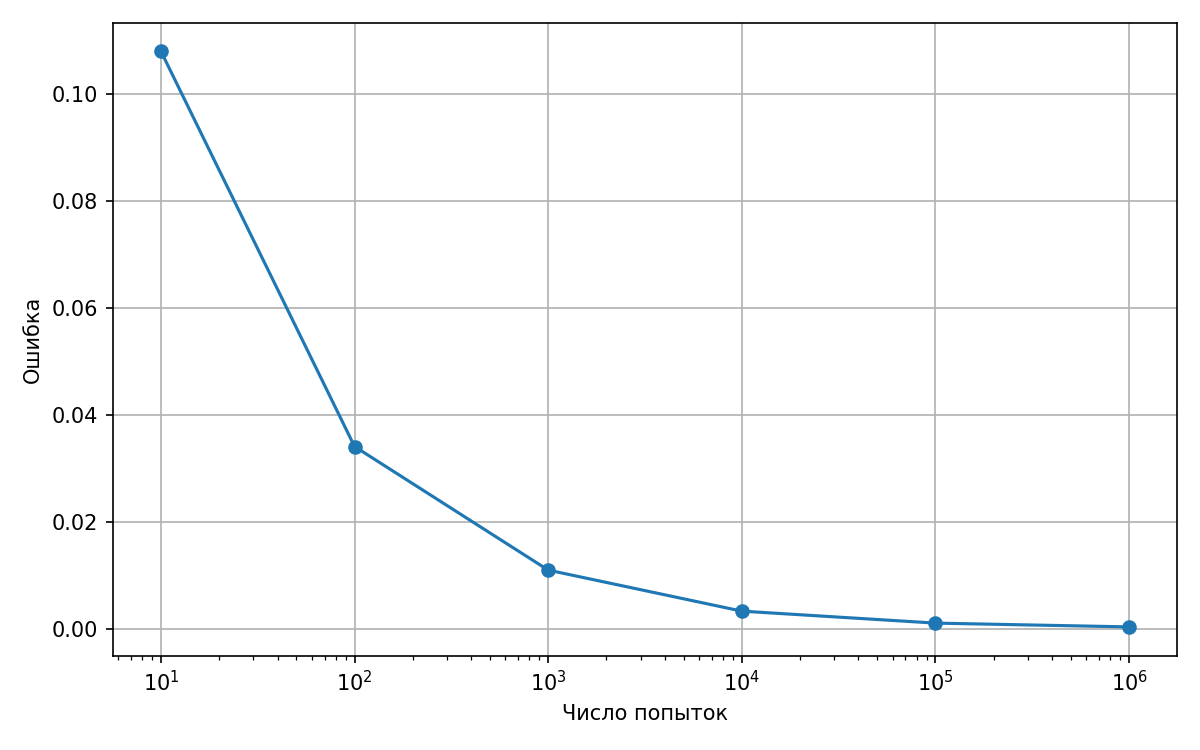
\includegraphics[width=0.82\textwidth]{average_error_plot.png}
\caption{Изменение средней абсолютной ошибки при увеличении числа испытаний}
\label{fig:error_graph}
\end{figure}

График показывает устойчивое уменьшение средней абсолютной ошибки при росте числа испытаний. При \texttt{TRIALS} = 10 средняя ошибка составляет $0.108008$, при \texttt{TRIALS} = 100 она уменьшается до $0.034069$, при \texttt{TRIALS} = 1000~--- до $0.010956$, а при \texttt{TRIALS} = 1000000 достигает значения $0.000332$. Наиболее заметное снижение ошибки наблюдается при переходе от малых значений \texttt{TRIALS} к средним, а при очень больших значениях уменьшение ошибки продолжается уже более плавно. Это соответствует ожидаемому поведению статистического моделирования: чем больше проведено испытаний, тем ближе экспериментальные оценки к аналитическим значениям.

Для классического случая задачи Монти Холла получены следующие оценки ошибок.

\begin{table}[H]
\centering
\small
\begin{tabular}{|c|c|c|c|c|}
\hline
\texttt{TRIALS} & Стратегия & Теоретическое значение & Полученное значение & Абсолютная ошибка \\
\hline
1000 & оставить & 0.333333 & 0.347000 & 0.013667 \\
\hline
1000 & сменить & 0.666667 & 0.679000 & 0.012333 \\
\hline
100000 & оставить & 0.333333 & 0.332220 & 0.001113 \\
\hline
100000 & сменить & 0.666667 & 0.668690 & 0.002023 \\
\hline
\end{tabular}
\caption{Проверка классического случая $N = 3$, $K = 1$}
\label{tab:monty_check}
\end{table}

Полученные значения подтверждают адекватность построенной модели: классический результат воспроизводится корректно, а увеличение числа испытаний приводит к уменьшению отклонения от теории. Результаты серии запусков показывают, что стратегия смены двери оказывается выгоднее стратегии сохранения выбора. При увеличении числа открытых пустых дверей $K$ преимущество смены выбора возрастает, поскольку игрок получает больше информации о положении приза. Зависимость вероятности выигрыша от $p_{\text{сохр}}$ имеет линейный характер: чем чаще игрок сохраняет первоначальный выбор, тем ближе итоговая вероятность выигрыша к $\frac{1}{N}$. В целом результаты статистического моделирования хорошо согласуются с аналитической формулой и подтверждают корректность построенной модели.

\section{Вывод}

В ходе работы была построена вероятностная модель обобщенной задачи Монти Холла и получена аналитическая формула для вероятности выигрыша игрока. Адекватность модели подтверждена на классическом случае при $N = 3$ и $K = 1$. Результаты вычислительного эксперимента хорошо согласуются с аналитическими значениями, а увеличение числа испытаний приводит к заметному уменьшению погрешности.

\section{Практическая реализация}

\refstepcounter{lstlisting}\label{lst:code}
\noindent Листинг~\ref{lst:code}. Исходный код программы.

\lstinputlisting[
    language=Python,
    frame=single
]{main.py}

\end{document}
